\documentclass{beamer}
\usepackage[slovene]{babel}
\usepackage[utf8]{inputenc}
\usepackage[T1]{fontenc}
\usepackage{lmodern}

\usetheme{CambridgeUS}
\setbeamertemplate{navigation symbols}{}

\newtheorem{thm}{Izrek}
\newtheorem{definicija}{Definicija}

\usepackage{amsmath}
\usepackage{graphicx}
\usepackage{amsfonts}

\title[Algoritem potisni-povišaj]{Algoritem potisni-povišaj za iskanje maksimalnih pretokov}
\subtitle{Zagovor dela diplomskega seminarja}
\author{Marcel Čampa}
\date{13. september 2018}
\institute[FMF UL]{Fakulteta za matematiko Univerze v Ljubljani}

\begin{document}

\begin{frame}
\maketitle
\end{frame}

\begin{frame}{Pregled vsebine}
\tableofcontents
\end{frame}


\section{Uvod}

\subsection{Osnovne definicije}
\begin{frame}{Graf in omrežje}
    \begin{definicija}
    \textbf{Graf} $G$ je par množic $G = (V,E)$, kjer je $V$ množica vozlišč grafa, $E \subseteq V \times V$ pa je množica usmerjenih povezav grafa $G$.
    \end{definicija}

    \begin{definicija}
    Naj bo $G = (V, E)$ graf. \textbf{Omrežje} na grafu $G$ je par $(G, c)$, kjer je $c \colon V \times V \rightarrow \mathbb{R}^+_0 \cup \{\infty\}$ \textbf{funkcija prepustnosti}, ki vsakemu paru vozlišč $(u,v)$ priredi prepustnost $c(u,v)$ povezave od $u$ do $v$. Prepustnost $c(u,v) = \infty$ natanko tedaj, ko prepustnost povezave ni omejena.

    Velja še, da $c(u,v)=0$ natanko tedaj, ko povezava ne obstaja v $G$.

    \textbf{Pretočno omrežje} na omrežju $(G,c)$ je četverica $(G,c,s,t)$, kjer je $s\in V$ začetno vozlišče pretočnega omrežja, rečemo mu \textbf{izvir}, $t\in V$ pa končno vozlišče pretočnega omrežja, ki mu pravimo \textbf{ponor}.
    \end{definicija}
\end{frame}

\begin{frame}{(Maksimalni) pretok}
    \begin{definicija}
    \textbf{Pretok} $f$ je tak psevdopretok, v katerem za vsak $v \in V \setminus\{s,t\}$ velja, da je neto tok, ki priteče v vozlišče $v$, enak nič, torej da velja $e_f(v) = 0$.
    \end{definicija}

    \begin{definicija}
    \textbf{Maksimalni pretok} je pretok $f$, za katerega velja \[|f| = \max_{f_i} |f_i|,\] kjer $f_i$ teče po vseh možnih pretokih skozi omrežje.
    \end{definicija}

\end{frame}

\subsection{Pregled algoritmov}
\begin{frame}{Pregled algoritmov}
    \centering
    \begin{tabular}{|l||l|l|}\hline
        \textit{algoritem} & \textit{časovna zahtevnost} & \textit{leto}\\\hline\hline
        linearno programiranje & &\\\hline
        Ford-Fulkerson & $\mathcal{O}(E \max|f|)$ & 1956 \\\hline
        Edmonds-Karp & $\mathcal{O}(V^2E)$ & 1972 \\\hline
        Dinic & $\mathcal{O}(VE \log V)$ & 1970 \\\hline
        potisni-povišaj (gen.) & $\mathcal{O}(V^2E)$ & 1986 \\\hline
        potisni-povišaj & $\mathcal{O}(V^3)$ & 1988 \\\hline
        KRT & $\mathcal{O}(VE \log_{\frac{E}{V \log V}} V)$ & 1994 \\\hline
        Orlin + KRT & $\mathcal{O}(VE)$ & 2013 \\\hline
    \end{tabular}
\end{frame}

\section{Algoritem potisni-povišaj}
\begin{frame}[fragile]{Osnovni algoritem}
\begin{verbatim}
POTISNI-POVIŠAJ(G,s)
1   INICIALIZIRAJ_PREDPRETOK(G,s)
2   DOKLER obstaja mogoča operacija POTISNI ali POVIŠAJ
3       izvedi mogočo operacijo
\end{verbatim}
\end{frame}

\begin{frame}[fragile]{Operacija \texttt{POTISNI}}
\begin{verbatim}
POTISNI (u, v)
1   // Potisnemo lahko, če je e(u) > 0,
2   // c_f(u,v) > 0 in h(u) = h(v) + 1.
3   delta = min{ e(u), c(u,v) - f(u,v) }
4   f(u,v) += delta
5   f(v,u) -= delta
6   e(u) -= delta
7   e(v) += delta
\end{verbatim}
\end{frame}

\begin{frame}[fragile]{Operacija \texttt{POVIŠAJ}}
\begin{verbatim}
POVIŠAJ (u)
1   // Vozlišče u povišamo, če je e(u) > 0 in
2   // za vsak v iz V, (u,v) v E_f, velja h(u) <= h(v).
3   h(u) = min{ h(v) : (u,v) v E_f } + 1
\end{verbatim}
\end{frame}

\begin{frame}[fragile]{Operacija \texttt{INICIALIZIRAJ\_PREDPRETOK}}
\begin{verbatim}
INICIALIZIRAJ_PREDPRETOK(G,s)
 1   // V grafu G z izbranim izvirom s
 2   // inicializiramo predpretok.
 3   ZA vsak v v V(G)
 4       h(v) = 0
 5       e(v) = 0
 6   ZA vsak (u,v) v E(G)
 7       f(u,v) = 0
 8   h(s) = |V|
 9   ZA vsak v, za katerega obstaja (s,v) v E(G)
10       f(s,v) = c(s,v)
11       f(v,s) = -f(s,v)
12       e(v) = f(s,v)
\end{verbatim}
\end{frame}


\section{Časovna zahtevnost}
\begin{frame}{Časovna zahtevnost}
    Število operacij
    \begin{itemize}
        \item \texttt{POTISNI} je kvečjemu $2|V||E| + 4|V|^2 (|V| + |E|)$;
        \item \texttt{POVIŠAJ} je kvečjemu $2|V|^2$.
    \end{itemize}
    \pause
    \begin{thm}
        Časovna zahtevnost algoritma \texttt{POTISNI-POVIŠAJ} je $\mathcal{O}(V^2E)$.
    \end{thm}
\end{frame}


\section{Zgled}
\begin{frame}{Začetno omrežje}
    \centering
    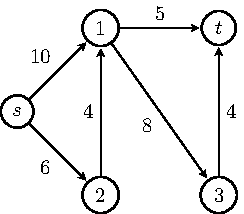
\includegraphics[scale=1.6]{../writing/images/graf2-1.pdf}
\end{frame}

\begin{frame}{Inicializacija predpretoka}
    \begin{columns}
        \begin{column}{0.5\textwidth}
            \centering
            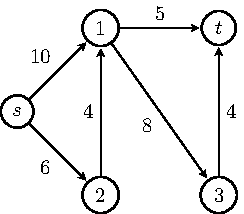
\includegraphics[scale=1.2]{../writing/images/graf2-1.pdf}
        \end{column}
        \pause
        \begin{column}{0.5\textwidth}
            \centering
            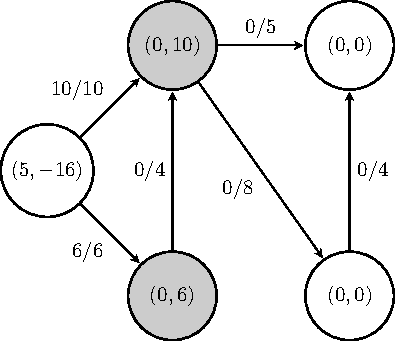
\includegraphics[scale=0.7]{../writing/images/graf2-2.pdf}
        \end{column}
    \end{columns}
\end{frame}

\begin{frame}{Korak 1}
    \begin{columns}
        \begin{column}{0.5\textwidth}
            \centering
            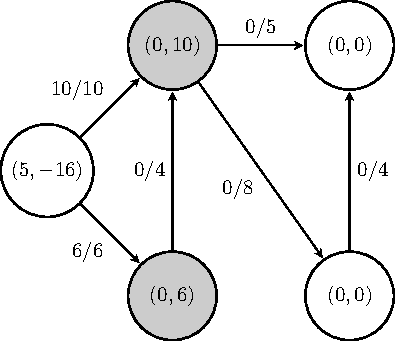
\includegraphics[scale=0.7]{../writing/images/graf2-2.pdf}
        \end{column}
        \pause
        \begin{column}{0.5\textwidth}
            \centering
            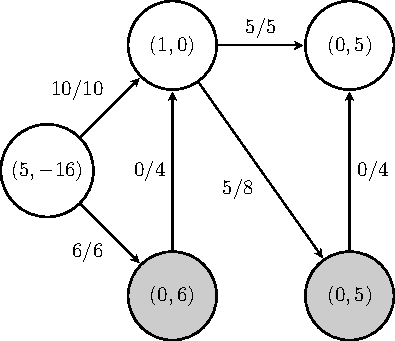
\includegraphics[scale=0.7]{../writing/images/graf2-3.pdf}
        \end{column}
    \end{columns}
\end{frame}

\begin{frame}{Korak 2}
    \begin{columns}
        \begin{column}{0.5\textwidth}
            \centering
            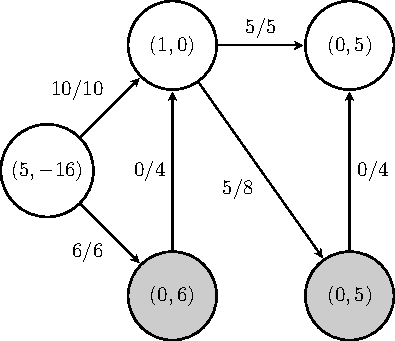
\includegraphics[scale=0.7]{../writing/images/graf2-3.pdf}
        \end{column}
        \pause
        \begin{column}{0.5\textwidth}
            \centering
            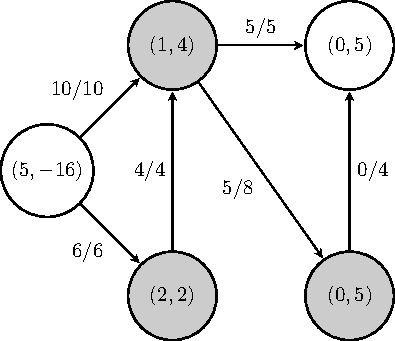
\includegraphics[scale=0.7]{../writing/images/graf2-4.pdf}
        \end{column}
    \end{columns}
\end{frame}

\begin{frame}{Korak 3}
    \begin{columns}
        \begin{column}{0.5\textwidth}
            \centering
            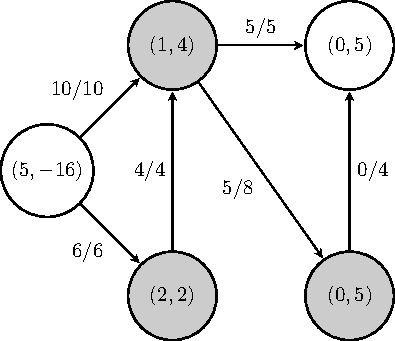
\includegraphics[scale=0.7]{../writing/images/graf2-4.pdf}
        \end{column}
        \pause
        \begin{column}{0.5\textwidth}
            \centering
            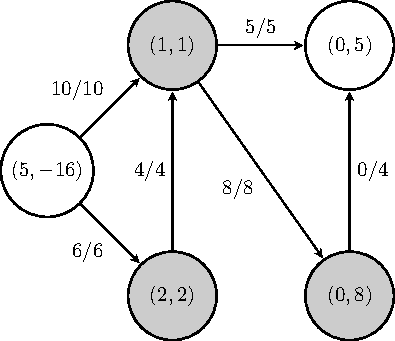
\includegraphics[scale=0.7]{../writing/images/graf2-5.pdf}
        \end{column}
    \end{columns}
\end{frame}

\begin{frame}{Korak 4}
    \begin{columns}
        \begin{column}{0.5\textwidth}
            \centering
            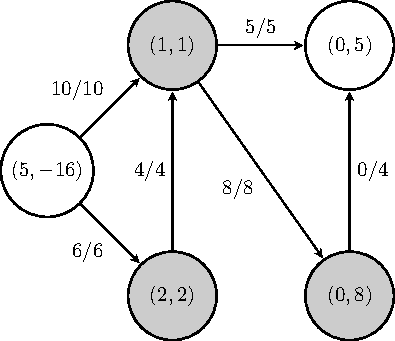
\includegraphics[scale=0.7]{../writing/images/graf2-5.pdf}
        \end{column}
        \pause
        \begin{column}{0.5\textwidth}
            \centering
            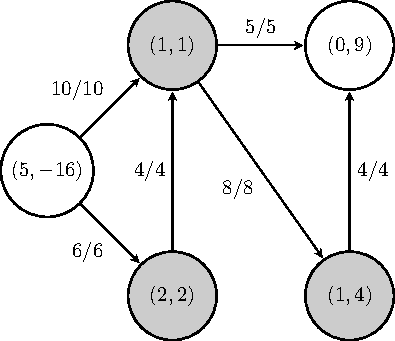
\includegraphics[scale=0.7]{../writing/images/graf2-6.pdf}
        \end{column}
    \end{columns}
\end{frame}

\begin{frame}{Korak 5}
    \begin{columns}
        \begin{column}{0.5\textwidth}
            \centering
            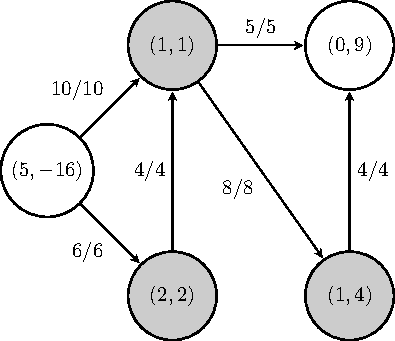
\includegraphics[scale=0.7]{../writing/images/graf2-6.pdf}
        \end{column}
        \pause
        \begin{column}{0.5\textwidth}
            \centering
            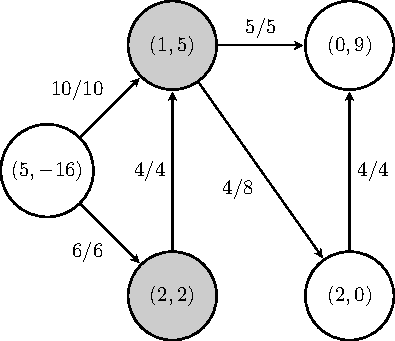
\includegraphics[scale=0.7]{../writing/images/graf2-7.pdf}
        \end{column}
    \end{columns}
\end{frame}

\begin{frame}{Korak 6}
    \begin{columns}
        \begin{column}{0.5\textwidth}
            \centering
            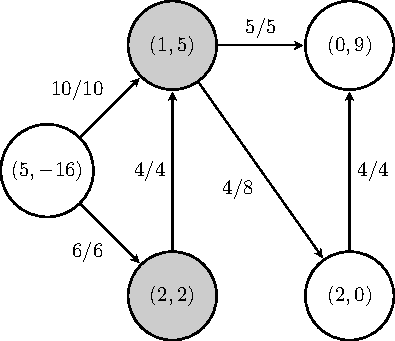
\includegraphics[scale=0.7]{../writing/images/graf2-7.pdf}
        \end{column}
        \pause
        \begin{column}{0.5\textwidth}
            \centering
            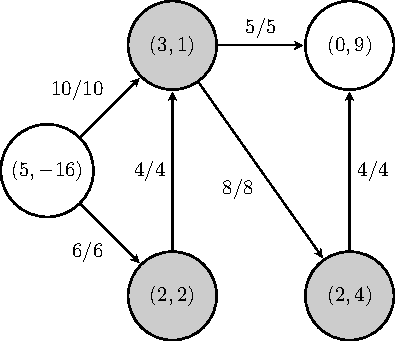
\includegraphics[scale=0.7]{../writing/images/graf2-8.pdf}
        \end{column}
    \end{columns}
\end{frame}

\begin{frame}{Korak 7}
    \begin{columns}
        \begin{column}{0.5\textwidth}
            \centering
            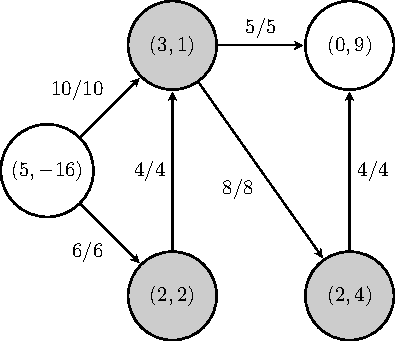
\includegraphics[scale=0.7]{../writing/images/graf2-8.pdf}
        \end{column}
        \pause
        \begin{column}{0.5\textwidth}
            \centering
            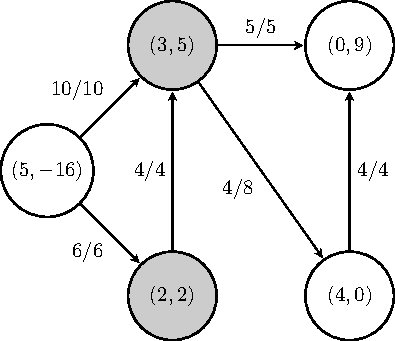
\includegraphics[scale=0.7]{../writing/images/graf2-9.pdf}
        \end{column}
    \end{columns}
\end{frame}

\begin{frame}{Korak 8}
    \begin{columns}
        \begin{column}{0.5\textwidth}
            \centering
            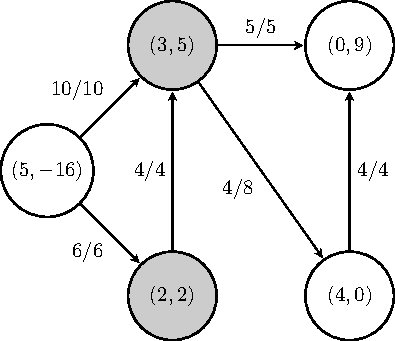
\includegraphics[scale=0.7]{../writing/images/graf2-9.pdf}
        \end{column}
        \pause
        \begin{column}{0.5\textwidth}
            \centering
            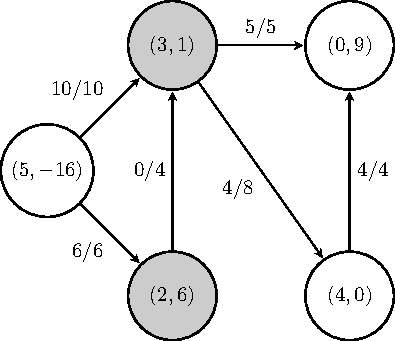
\includegraphics[scale=0.7]{../writing/images/graf2-10.pdf}
        \end{column}
    \end{columns}
\end{frame}

\begin{frame}{Korak 9}
    \begin{columns}
        \begin{column}{0.5\textwidth}
            \centering
            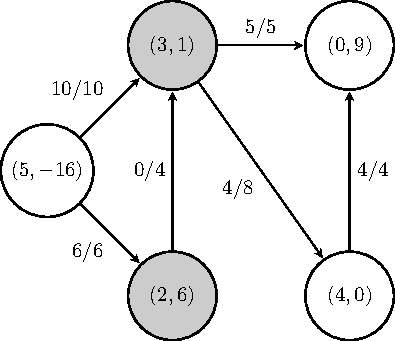
\includegraphics[scale=0.7]{../writing/images/graf2-10.pdf}
        \end{column}
        \pause
        \begin{column}{0.5\textwidth}
            \centering
            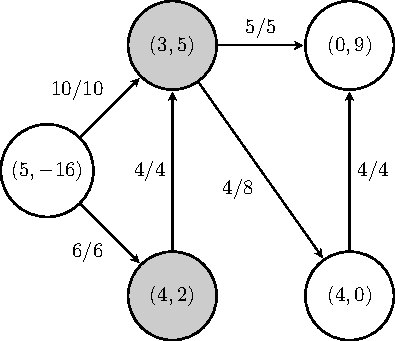
\includegraphics[scale=0.7]{../writing/images/graf2-11.pdf}
        \end{column}
    \end{columns}
\end{frame}

\begin{frame}{Korak 10}
    \begin{columns}
        \begin{column}{0.5\textwidth}
            \centering
            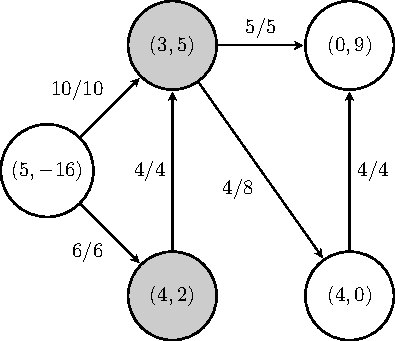
\includegraphics[scale=0.7]{../writing/images/graf2-11.pdf}
        \end{column}
        \pause
        \begin{column}{0.5\textwidth}
            \centering
            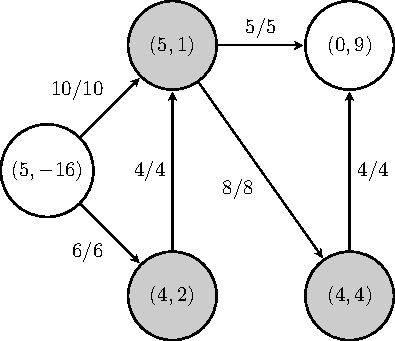
\includegraphics[scale=0.7]{../writing/images/graf2-12.pdf}
        \end{column}
    \end{columns}
\end{frame}

\begin{frame}{Korak 11}
    \begin{columns}
        \begin{column}{0.5\textwidth}
            \centering
            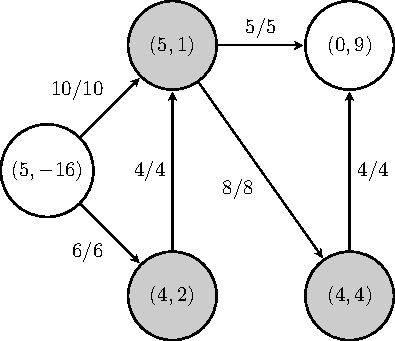
\includegraphics[scale=0.7]{../writing/images/graf2-12.pdf}
        \end{column}
        \pause
        \begin{column}{0.5\textwidth}
            \centering
            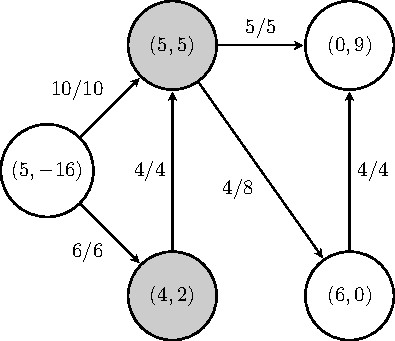
\includegraphics[scale=0.7]{../writing/images/graf2-13.pdf}
        \end{column}
    \end{columns}
\end{frame}

\begin{frame}{Korak 12}
    \begin{columns}
        \begin{column}{0.5\textwidth}
            \centering
            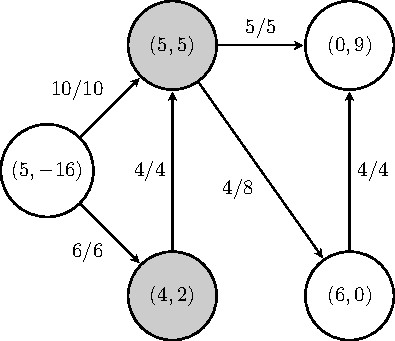
\includegraphics[scale=0.7]{../writing/images/graf2-13.pdf}
        \end{column}
        \pause
        \begin{column}{0.5\textwidth}
            \centering
            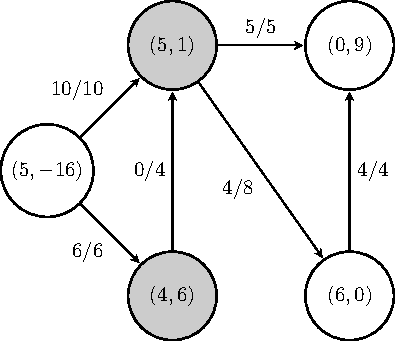
\includegraphics[scale=0.7]{../writing/images/graf2-14.pdf}
        \end{column}
    \end{columns}
\end{frame}

\begin{frame}{Korak 13}
    \begin{columns}
        \begin{column}{0.5\textwidth}
            \centering
            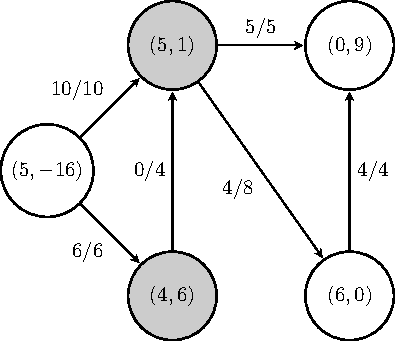
\includegraphics[scale=0.7]{../writing/images/graf2-14.pdf}
        \end{column}
        \pause
        \begin{column}{0.5\textwidth}
            \centering
            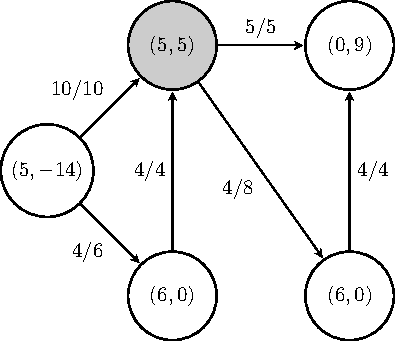
\includegraphics[scale=0.7]{../writing/images/graf2-15.pdf}
        \end{column}
    \end{columns}
\end{frame}

\begin{frame}{Korak 14}
    \begin{columns}
        \begin{column}{0.5\textwidth}
            \centering
            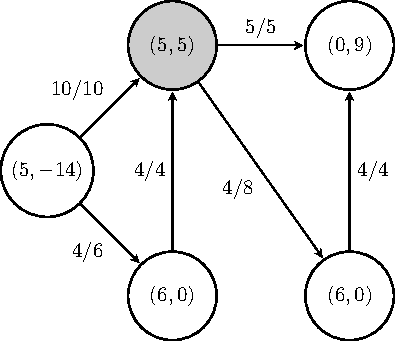
\includegraphics[scale=0.7]{../writing/images/graf2-15.pdf}
        \end{column}
        \pause
        \begin{column}{0.5\textwidth}
            \centering
            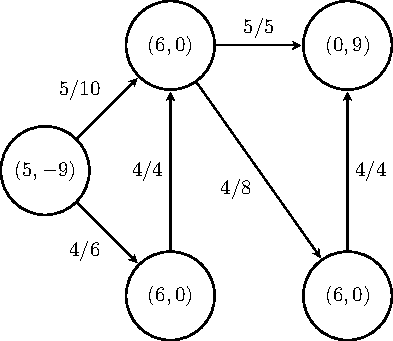
\includegraphics[scale=0.7]{../writing/images/graf2-16.pdf}
        \end{column}
    \end{columns}
\end{frame}

\section{Uporaba}
\begin{frame}{Problem ponudbe in povpraševanja}
    \centering\pause
    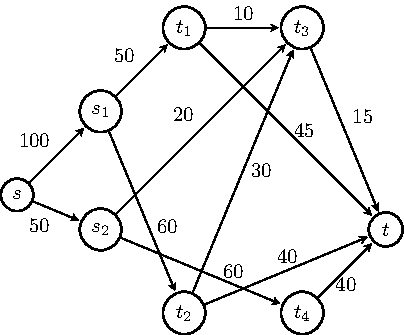
\includegraphics[scale=0.7]{../writing/images/primer1-1.pdf}~~~\pause
    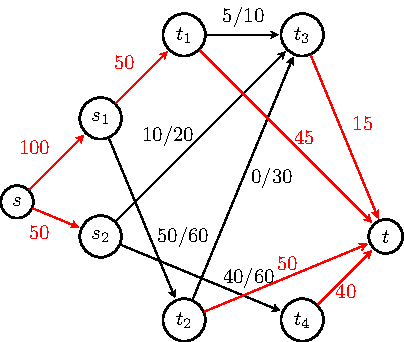
\includegraphics[scale=0.7]{../writing/images/primer1-3.pdf}
\end{frame}


\begin{frame}{Baseball elimination}
    \centering\pause
    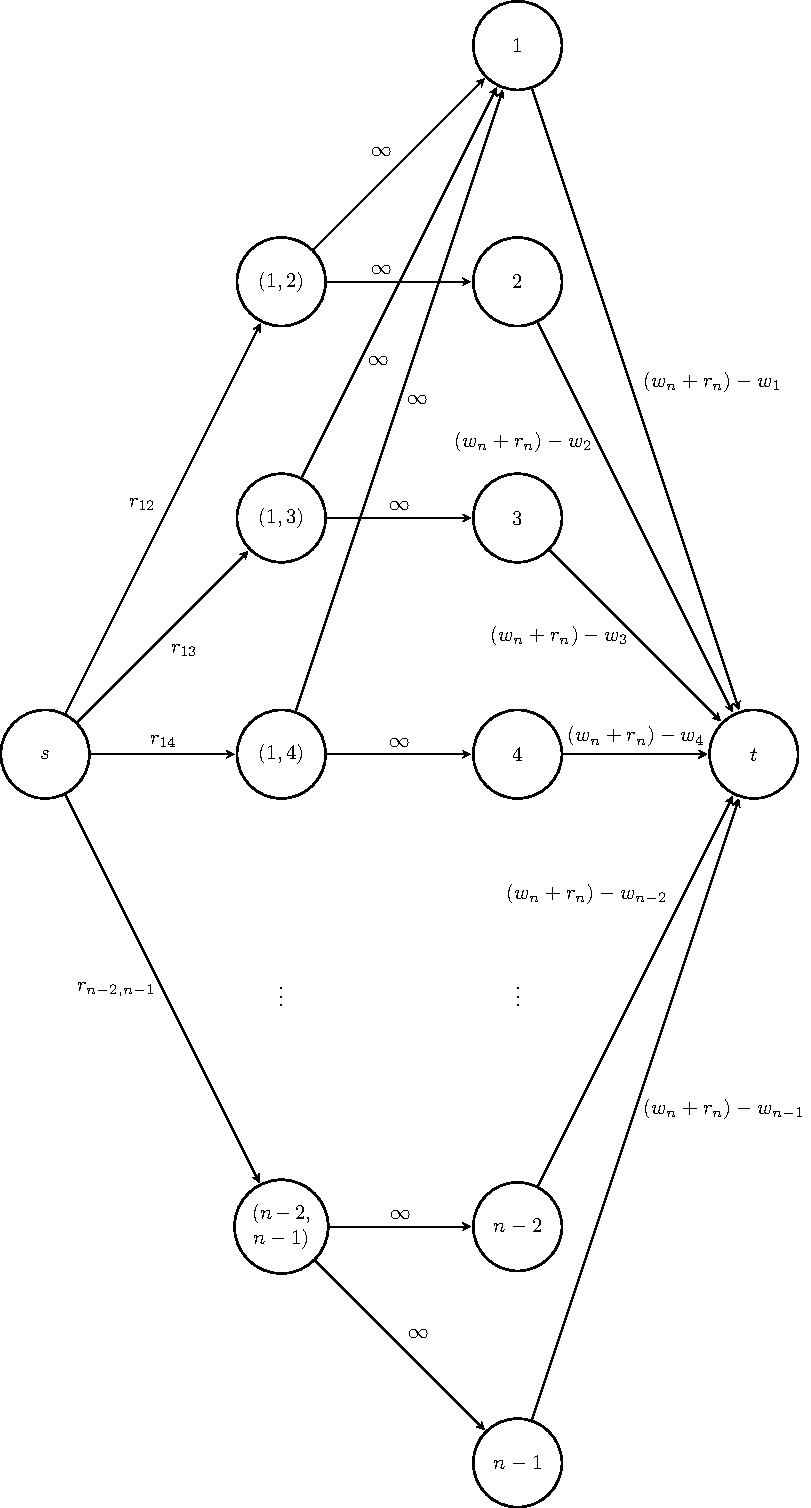
\includegraphics[scale=0.3]{../writing/images/baseball1.pdf}
\end{frame}


\bgroup
\setbeamercolor{background canvas}{bg=black}
\begin{frame}[plain]{}
\end{frame}
\egroup




\end{document}
